%%!TEX root=../main.tex

\section{Experiments}

\subsection{Convolution Dictionary Learning (CDL) Experiments}
As mentioned in the background section, we want to try out different
learning algorithm mainly comparing the difference between with and
without consensus update. All of the sparse representation related 
experiments are done on a computer running Ubuntu 19 with a Intel 
i7-6700K CPU with 8 threads.
From the experiments we have chosen to use the province training 
data with 2223 20x20 gray-scale images. Both algorithms will 
attempt to build a dictionary with 25 channels of 4x4 filters.

Before running either of the algorithms, the images are being feed
into a Tikhonov Filter to extract their respective High-Pass and Low-Pass
components. An example is illustrated in Figure \ref{fig_CBRPDN_CSC_LHS_comp} and 
\ref{fig_CBRPDN_FISTA_LHS_comp}. 

Figure \ref{fig_CBRPDN_function_iter_plot} and \ref{fig_CCBRPDN_function_iter_plot}
shows that we stop when the functional value of the BRPDN has been stabilized.
Both algorithms runs for 200 iterations. However, the algorithm with consensus update
takes only 187.18s while the other one takes 499.37s. 
Figures \ref{fig_CBRPDN_Dict} and \ref{fig_CCBRPDN_Dict} shows that both resulting 
dictionaries are similar visually meaning that consensus method provide 
a 62.52\% reduction in runtime without a significant reduction in the 
quality of the resulting dictionary.

\begin{figure}[ht]
\centering
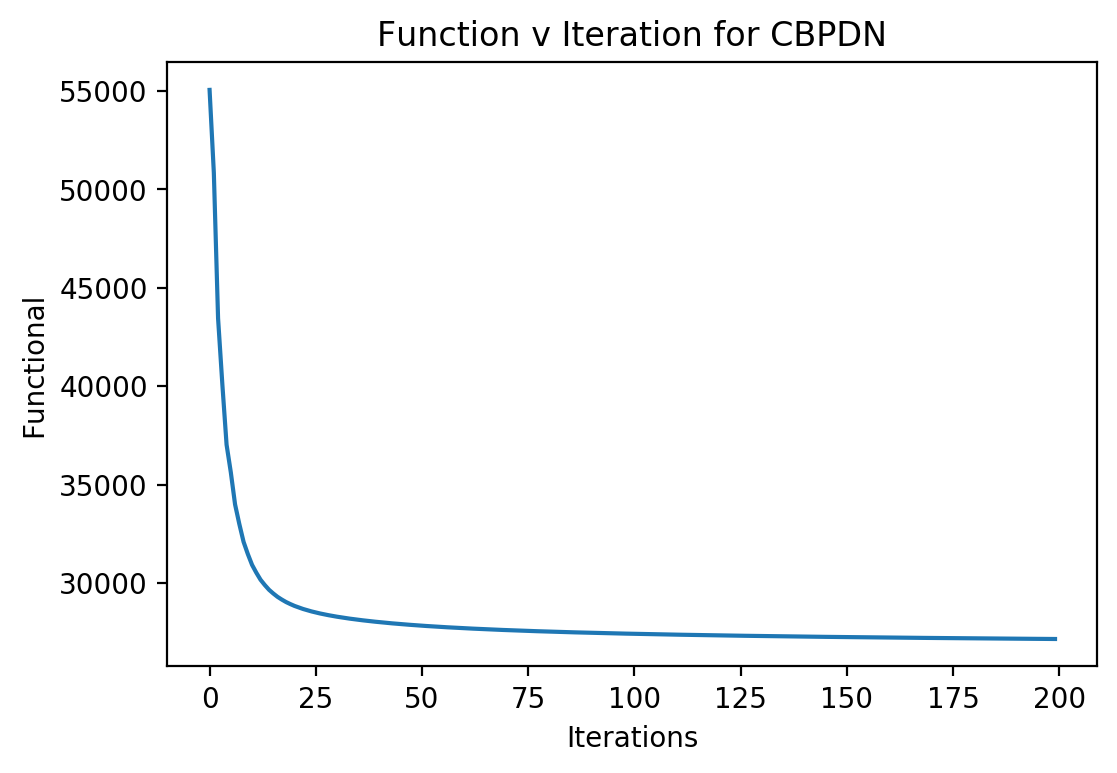
\includegraphics[width=2.5in]{\FIGDIR/CDL_CSC_plot/CBRPDN_function_iter_plot.png}
\caption{Functional Value against Iteration Plot without consensus}
\label{fig_CBRPDN_function_iter_plot}
\end{figure}

\begin{figure}[ht]
\centering
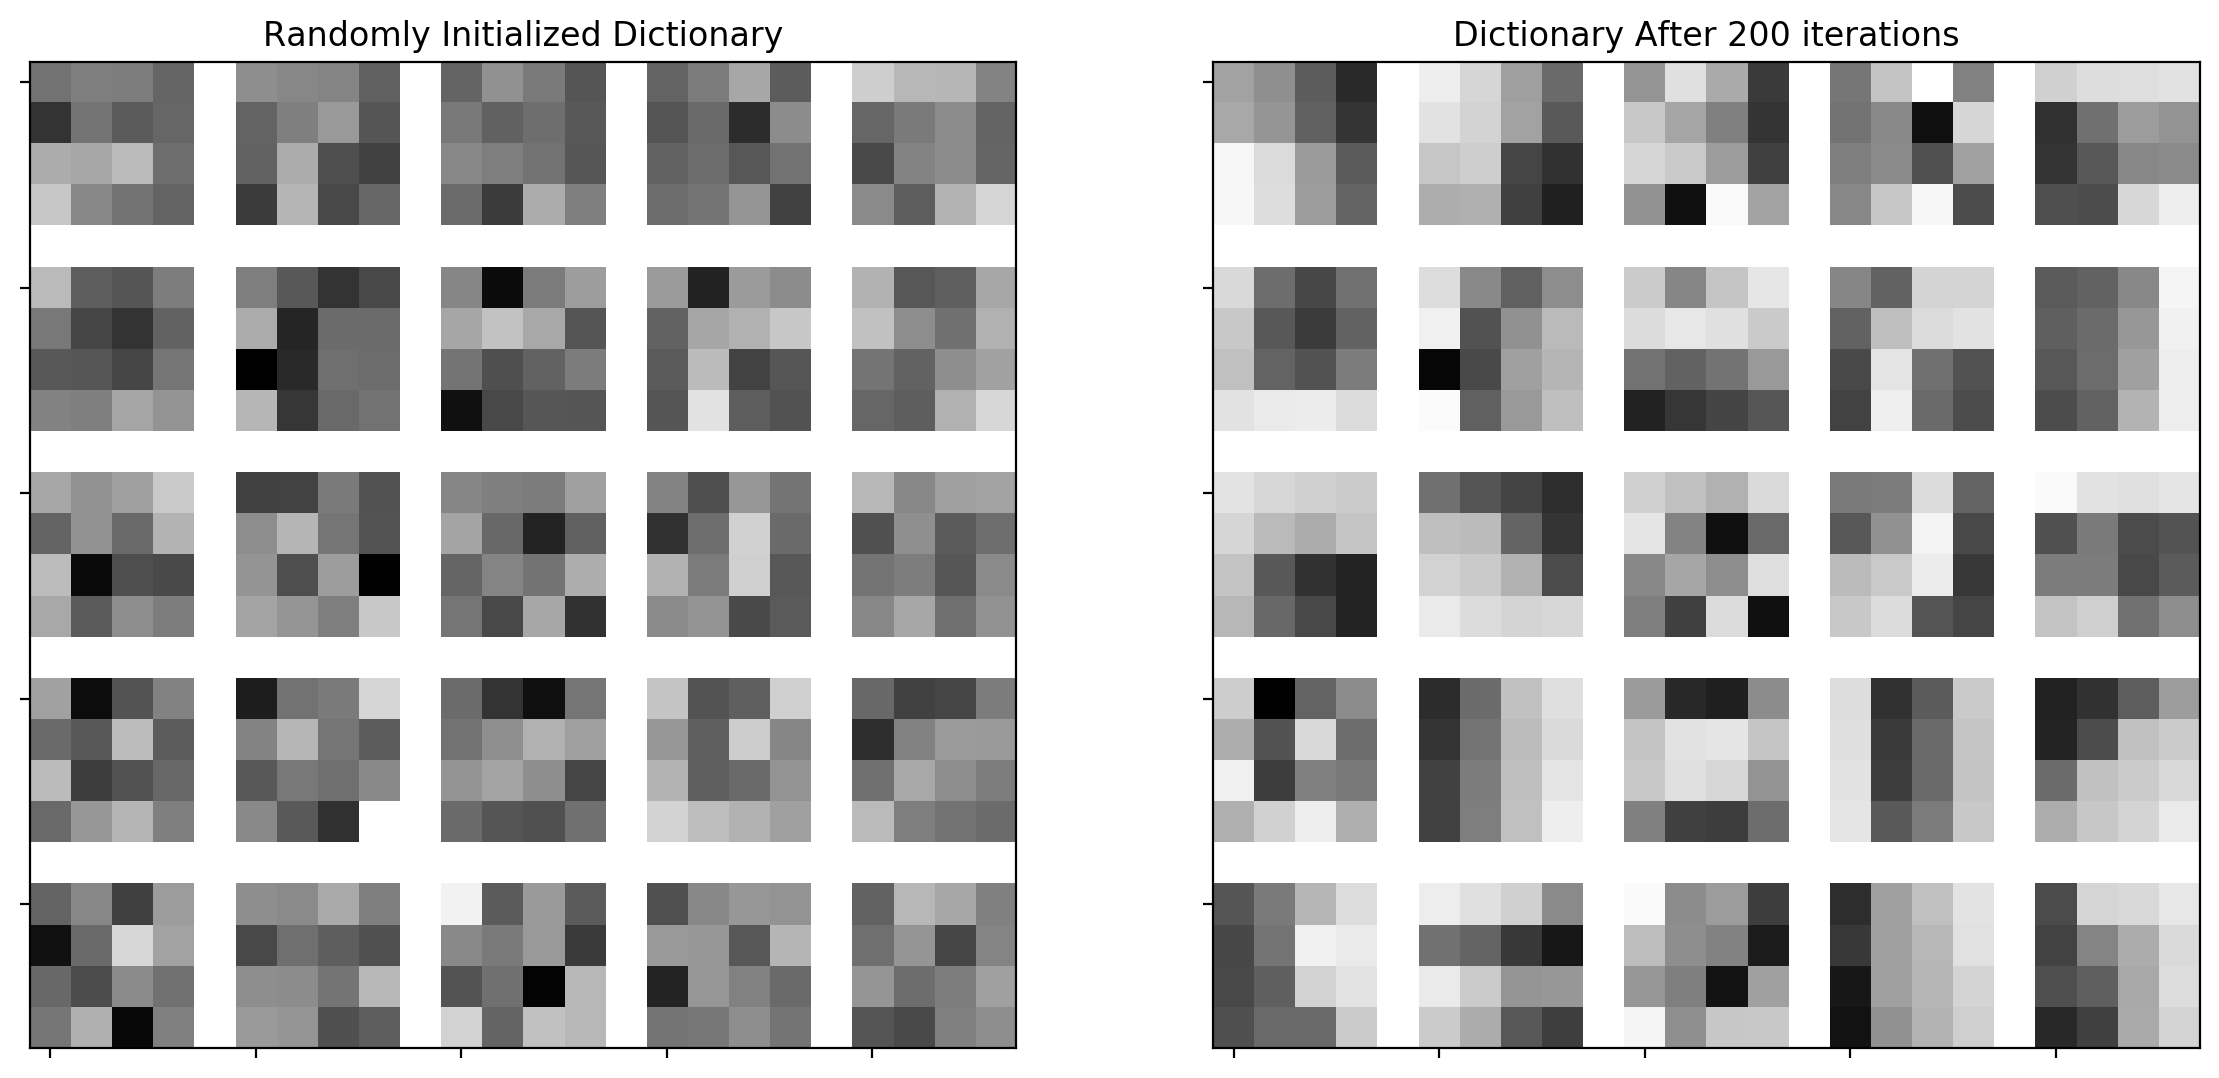
\includegraphics[width=2.5in]{\FIGDIR/CDL_CSC_plot/CBRPDN_Dict.png}
\caption{Resulting Dictionary without consensus}
\label{fig_CBRPDN_Dict}
\end{figure}

\begin{figure}[ht]
\centering
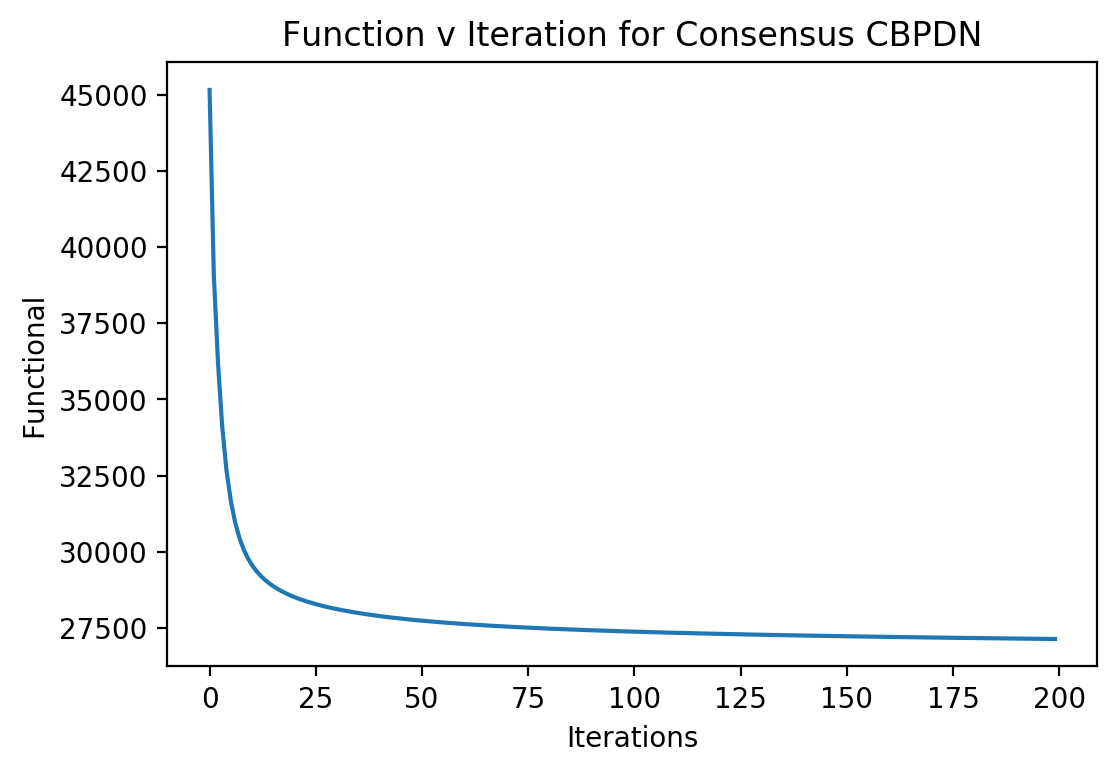
\includegraphics[width=2.5in]{\FIGDIR/CDL_CSC_plot/CCBRPDN_function_iter_plot.png}
\caption{Functional Value against Iteration Plot with consensus}
\label{fig_CCBRPDN_function_iter_plot}
\end{figure}

\begin{figure}[ht]
\centering
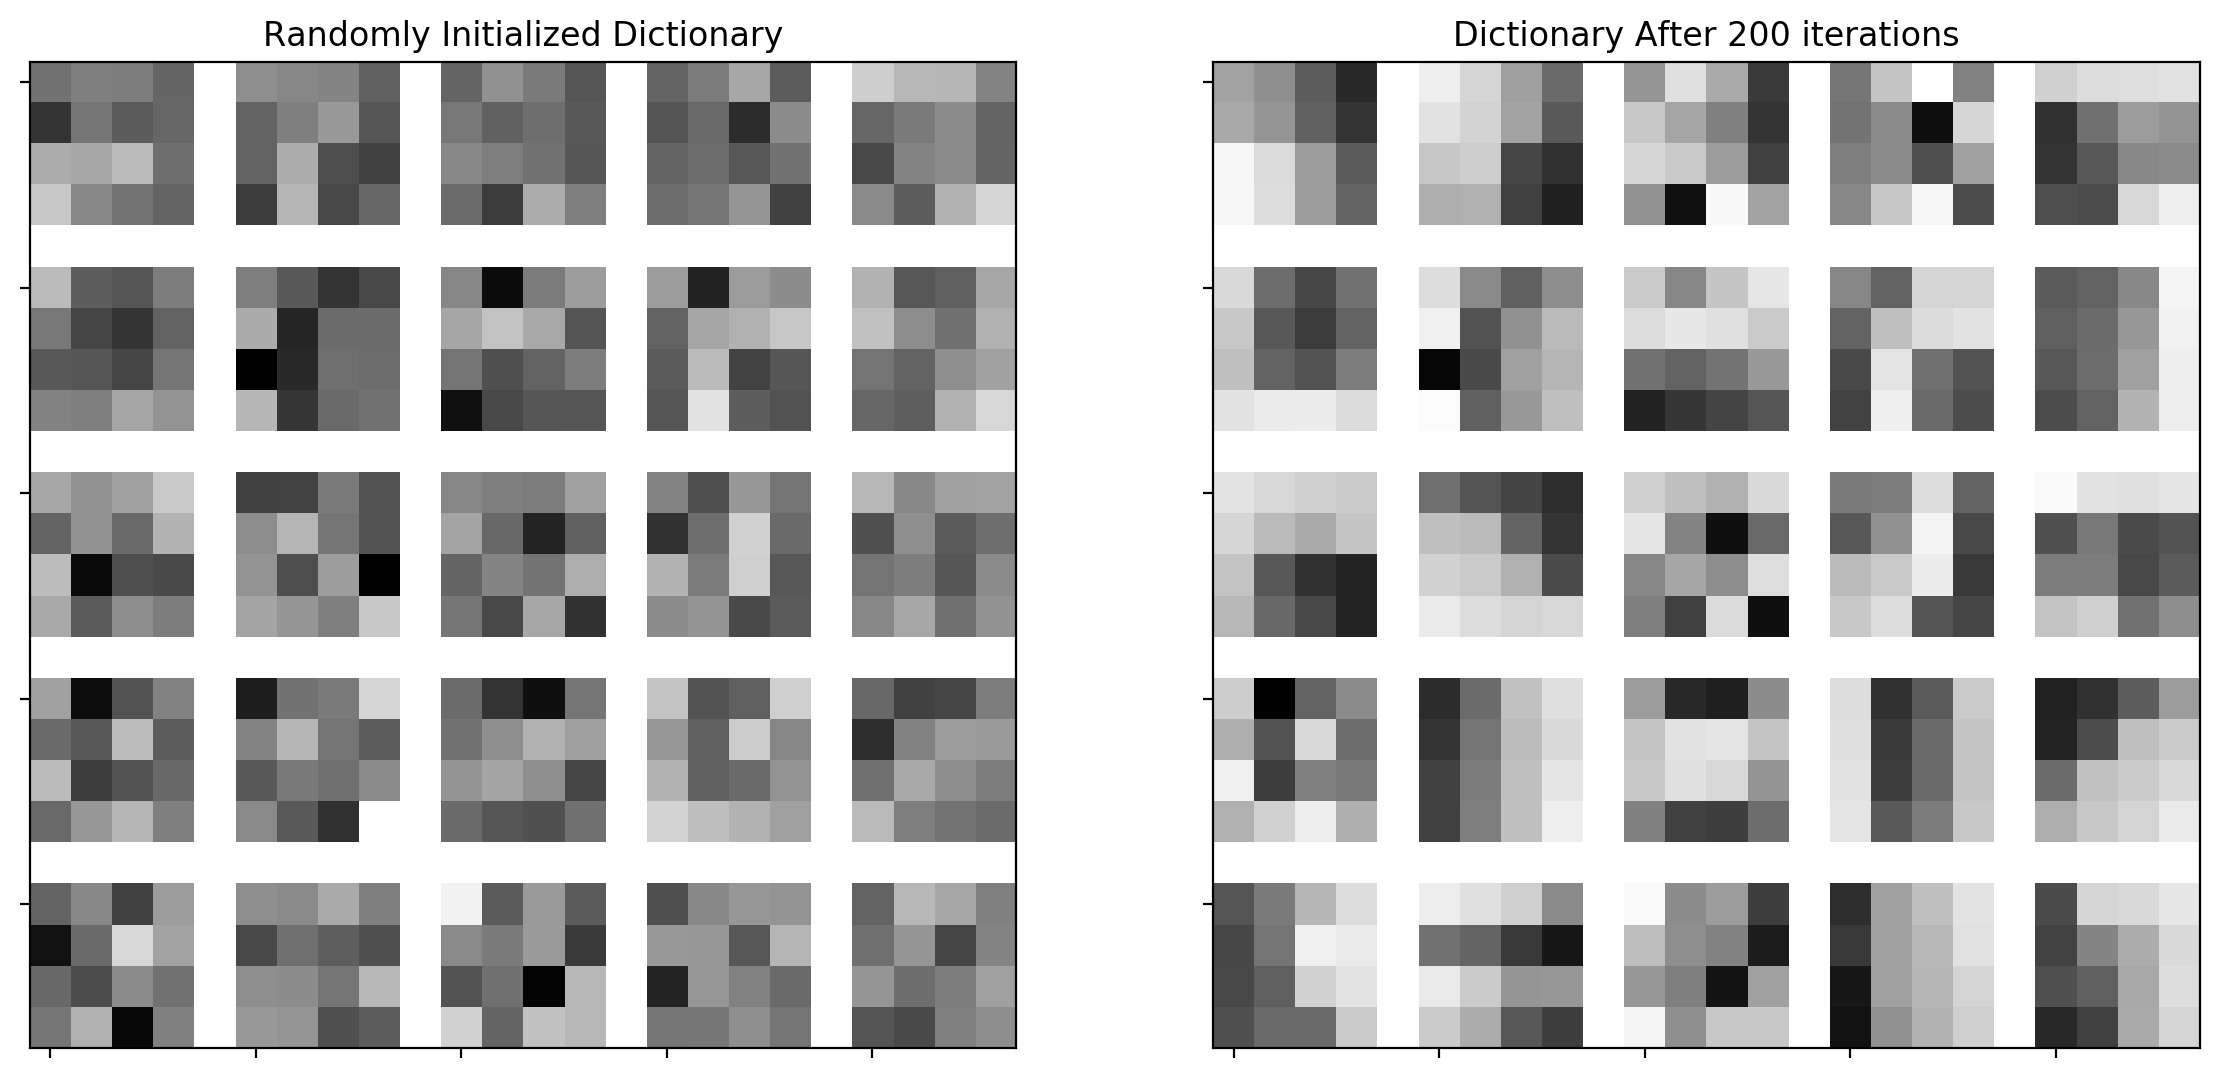
\includegraphics[width=2.5in]{\FIGDIR/CDL_CSC_plot/CCBRPDN_Dict.png}
\caption{Resulting Dictionary with consensus}
\label{fig_CCBRPDN_Dict}
\end{figure}

Since the CDL algorithm with consensus update save a significant amount of 
time, the dictionary generated using this algorithm has been chosen
as the dictionary to solve for the CSC problem. However side experiment has
also shown that the reconstruction Peak Signal-to-Noise Ration (PSNR) using 
the dictionary generated using the CDL with consensus has a lower value than 
the one using CDL without consensus when single-channel CSC is being used.
Under the same codex of the image, a higher PSRN value usually means
a better reconstruction of the image

\subsection{Convolution Sparse Coding (CSC) Experiments}
In order to solve for a sparse representation for each of the images, we 
have tested 2 algorithms before applying it to the full dataset.

Similar to CDL, the images are being feed into a Tikhonov Filter to extract
their respective High-Pass and Low-Pass components.

Comparing the runtime of single-channel CSC and the FISTA method, the 
FISTA methods run 10 times faster than the single-channel CSC method. The 
FISTA cost around 0.01s while single-channel CSC cost around 0.1s. However,
as shown in Figure \ref{fig_CCBRPDN_FISTA_recon} and \ref{fig_CBRPDN_FISTA_recon},
the reconstruction of the image is not as good as the reconstruction shown in
Figure \ref{fig_CCBRPDN_CSC_recon} and \ref{fig_CBRPDN_CSC_recon} which use the single 
channel CSC method. The PSRN value using the single channel CSC method is around 23-25 dB
which is always higher than 18.49 dB using the FISTa method.

On top of that, when we compare 
Figures \ref{fig_CBRPDN_CSC_LHS_comp} and \ref{fig_CCBRPDN_CSC_LHS_comp} as a set to
Figures \ref{fig_CBRPDN_FISTA_LHS_comp} and \ref{fig_CCBRPDN_FISTA_LHS_comp}, we can see that 
the sparse representation generated using the faster FISTA method is more noisy
and less sparse.

\begin{figure}
\centering
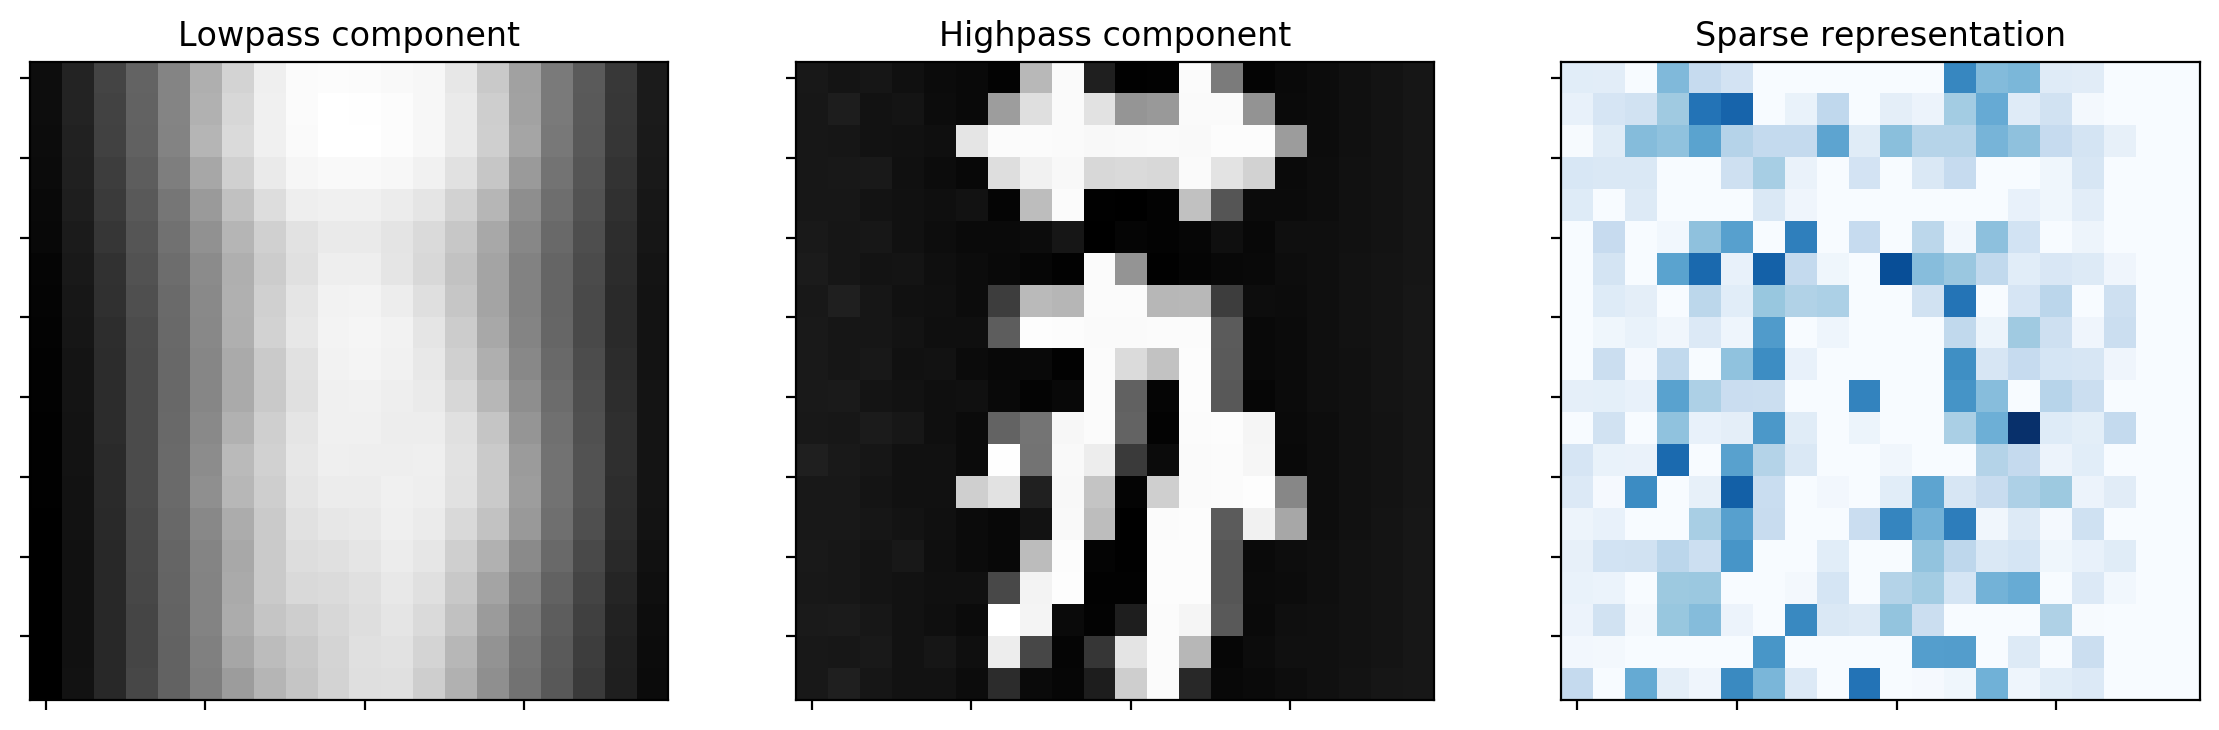
\includegraphics[width=2.5in]{\FIGDIR/CDL_CSC_plot/CBRPDN_CSC_LHS_comp.png}
\caption{Lowpass, Highpass and Parse representation using single channel CSC with non-consensus dictionary}
\label{fig_CBRPDN_CSC_LHS_comp}
\end{figure}

\begin{figure}
\centering
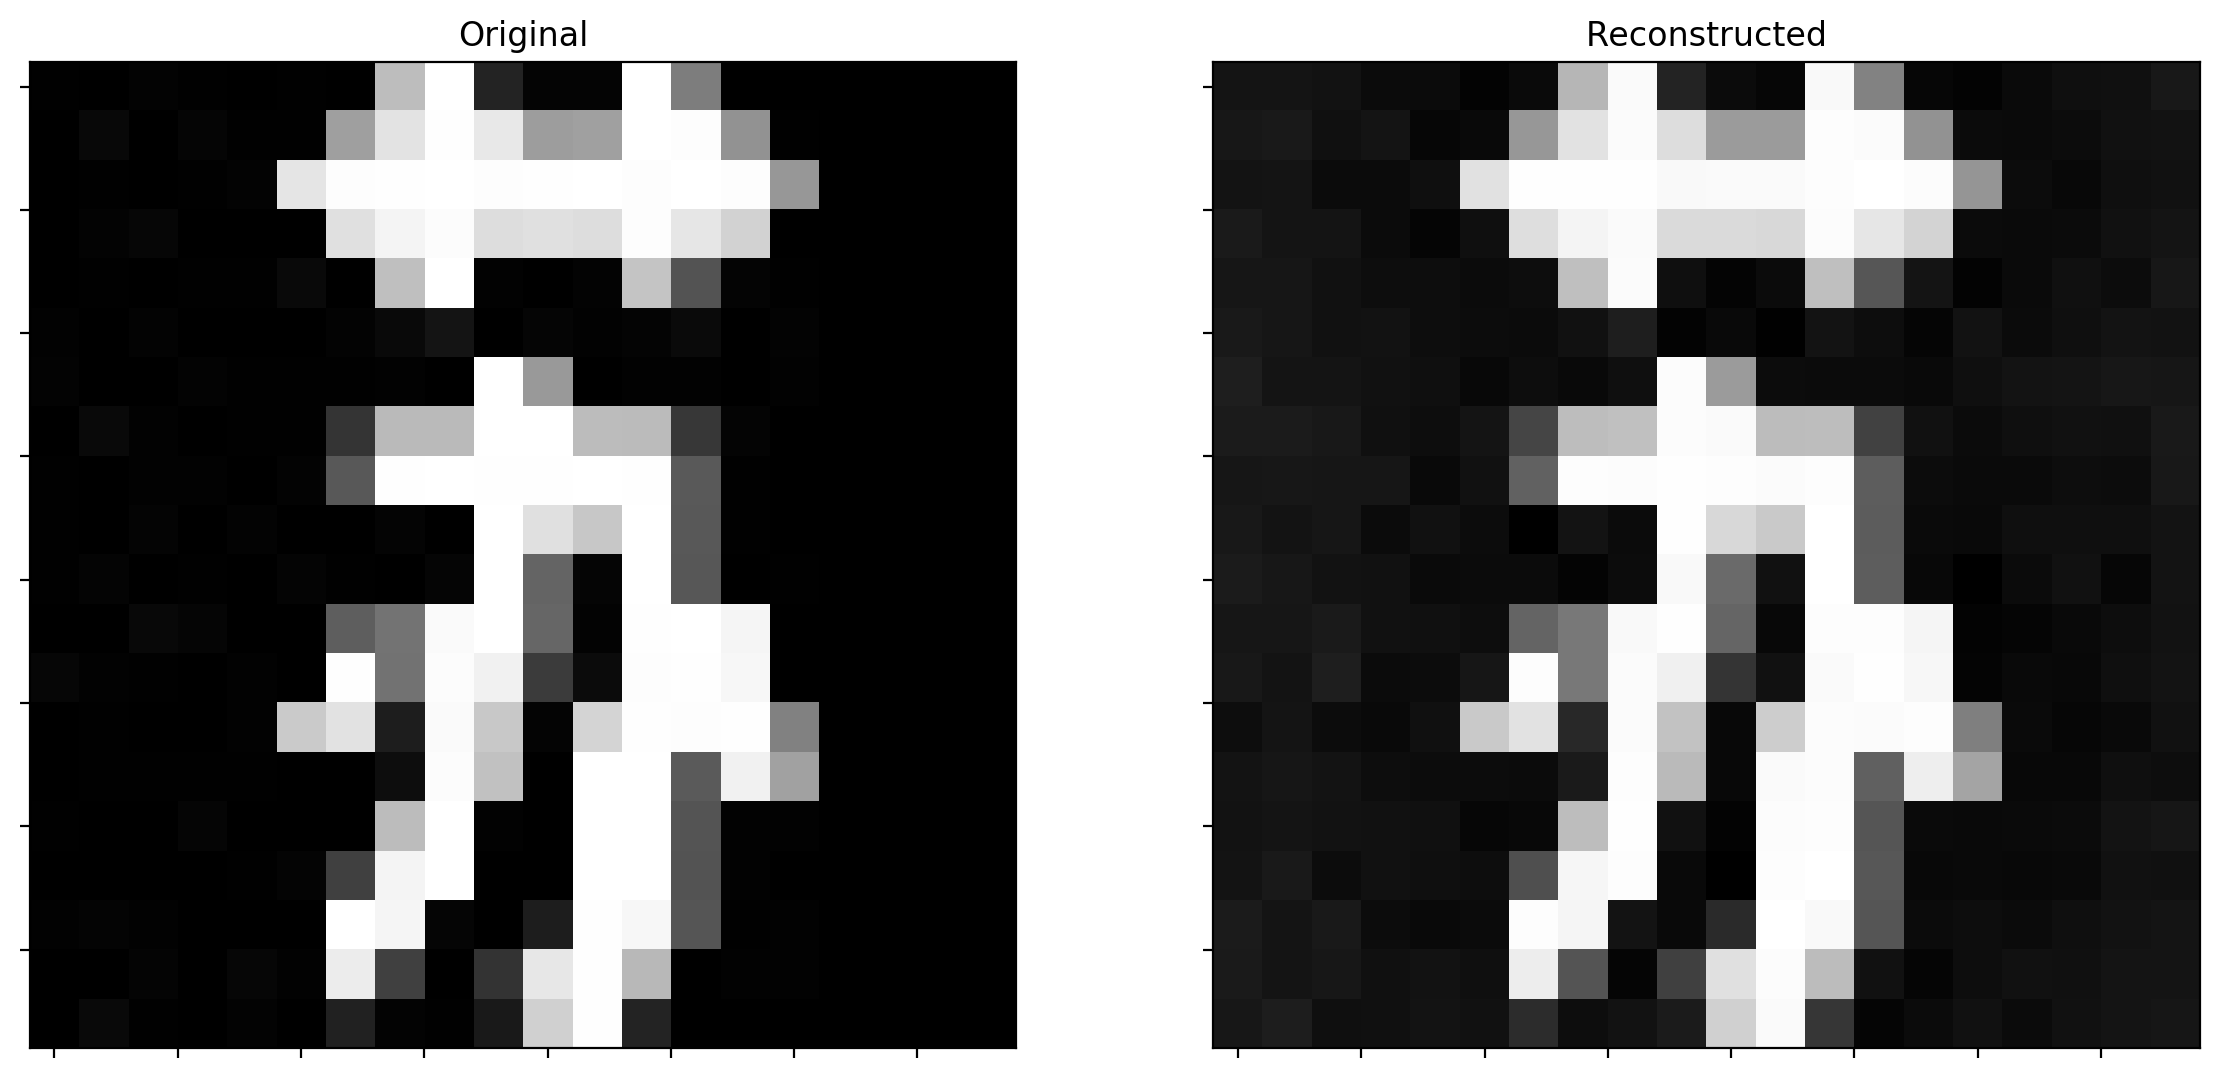
\includegraphics[width=2.5in]{\FIGDIR/CDL_CSC_plot/CBRPDN_CSC_recon.png}
\caption{Image Reconstruction using single channel CSC with non-consensus dictionary}
\label{fig_CBRPDN_CSC_recon}
\end{figure}

\begin{figure}
\centering
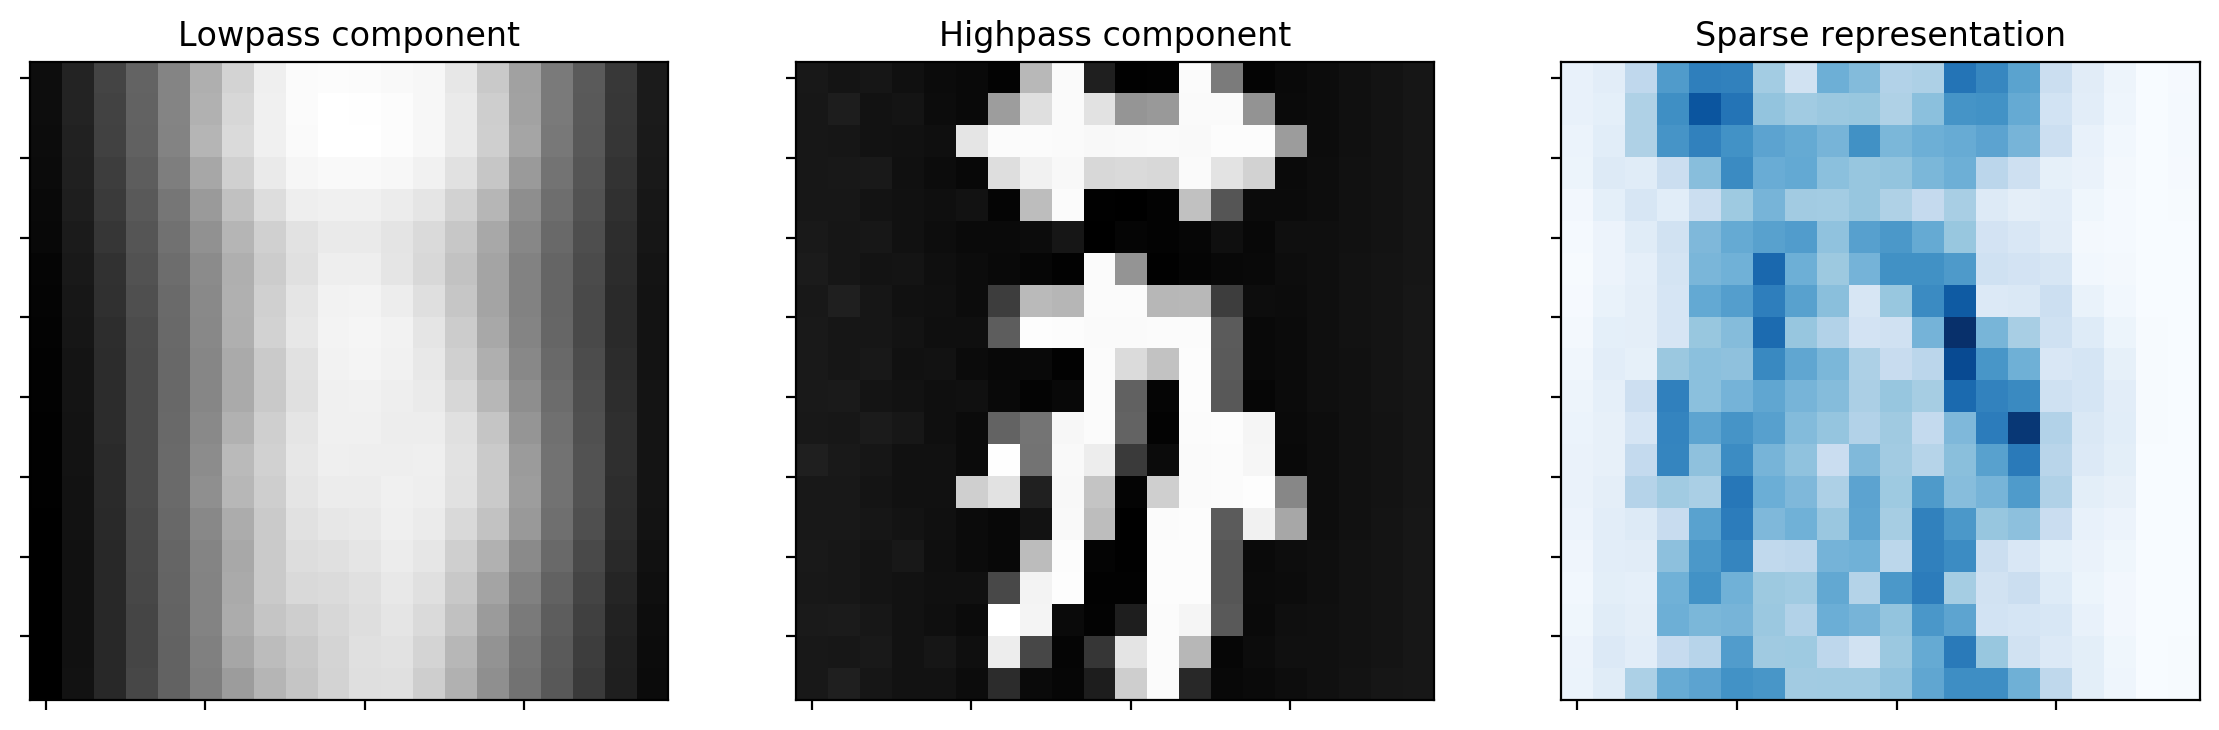
\includegraphics[width=2.5in]{\FIGDIR/CDL_CSC_plot/CBRPDN_FISTA_LHS_comp.png}
\caption{Lowpass, Highpass and Parse representation using FISTA CSC with non-consensus dictionary}
\label{fig_CBRPDN_FISTA_LHS_comp}
\end{figure}

\begin{figure}
\centering
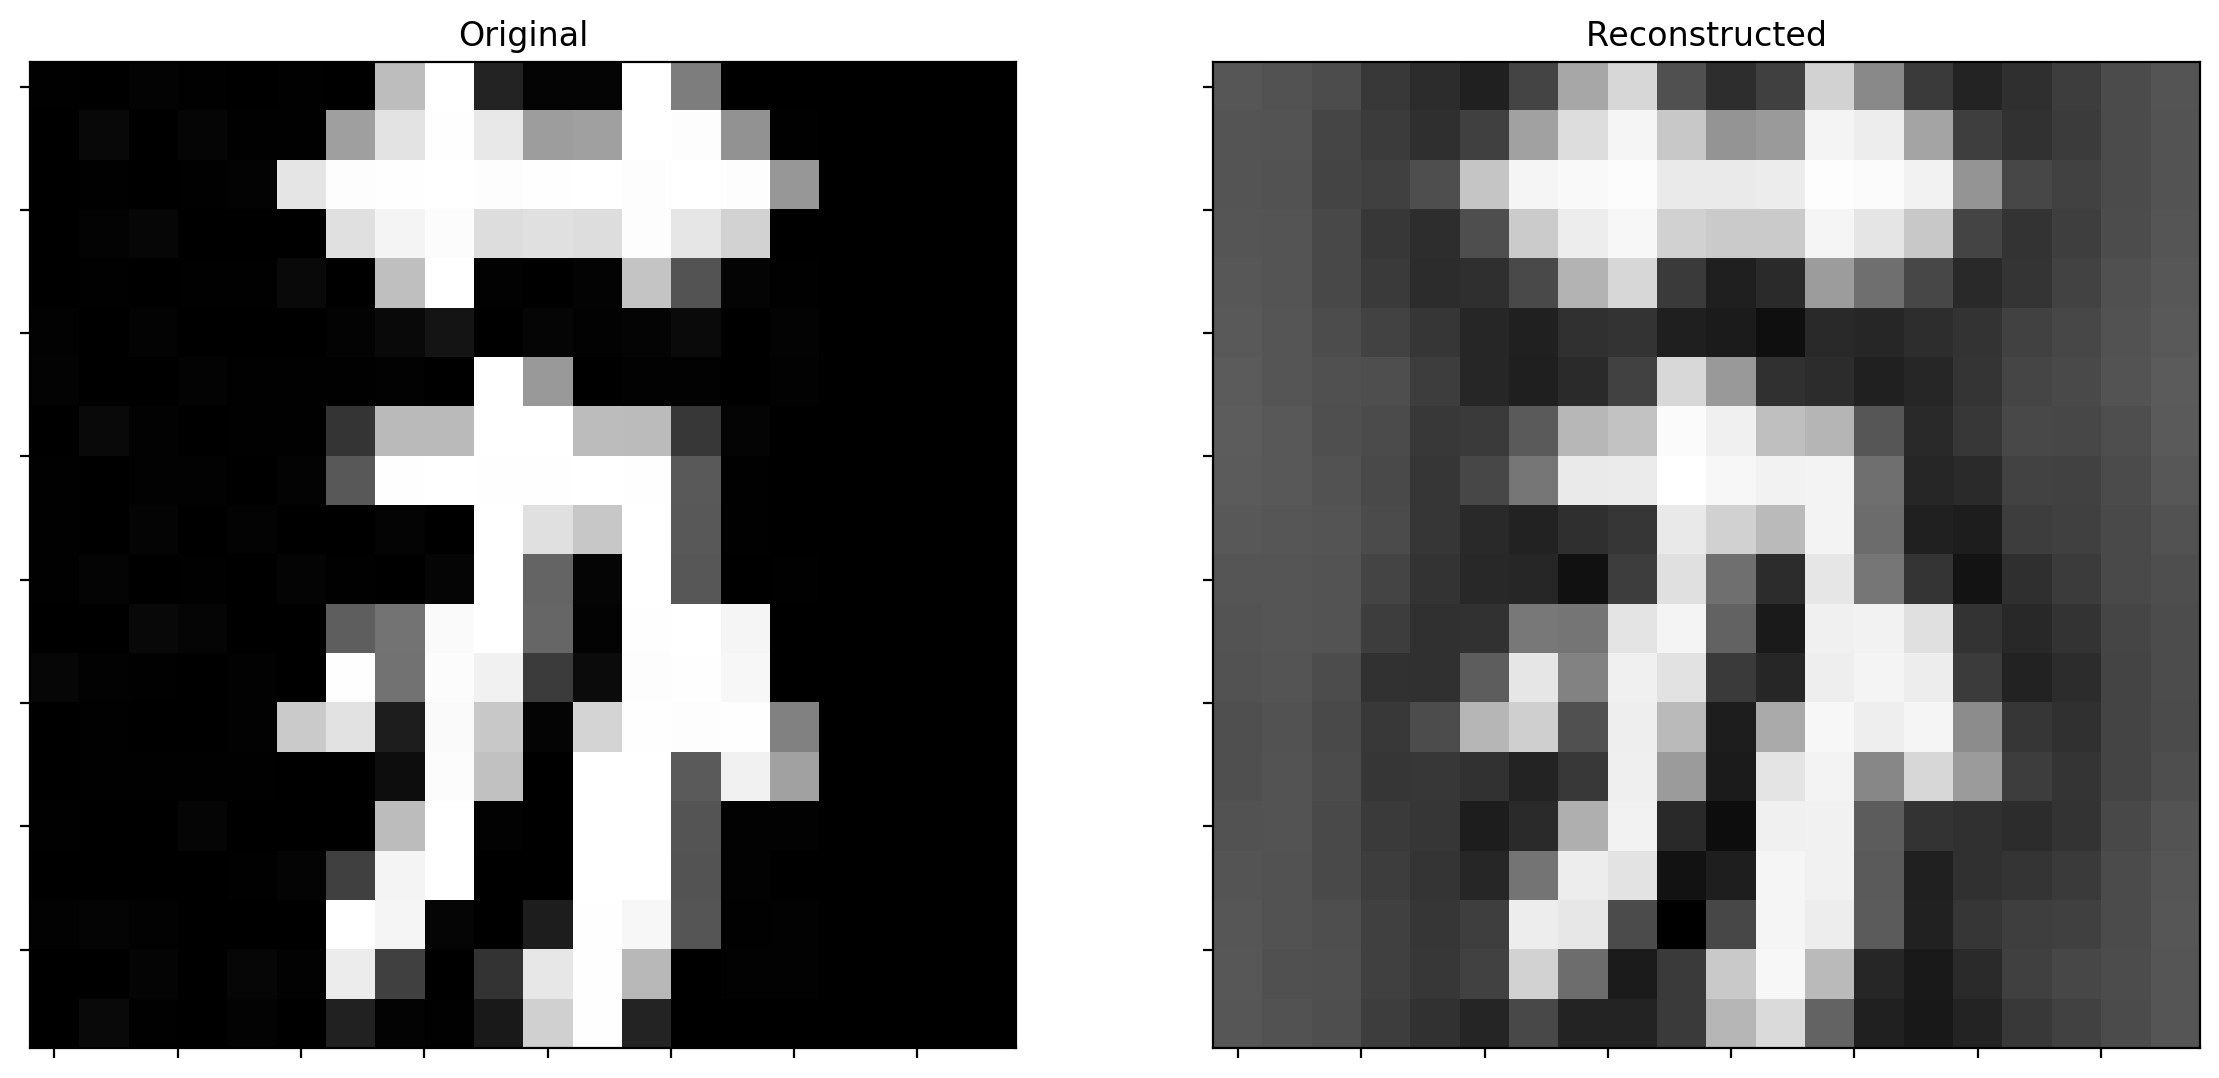
\includegraphics[width=2.5in]{\FIGDIR/CDL_CSC_plot/CBRPDN_FISTA_recon.png}
\caption{Image Reconstruction using FISTA CSC with non-consensus dictionary}
\label{fig_CBRPDN_FISTA_recon}
\end{figure}

\begin{figure}
\centering
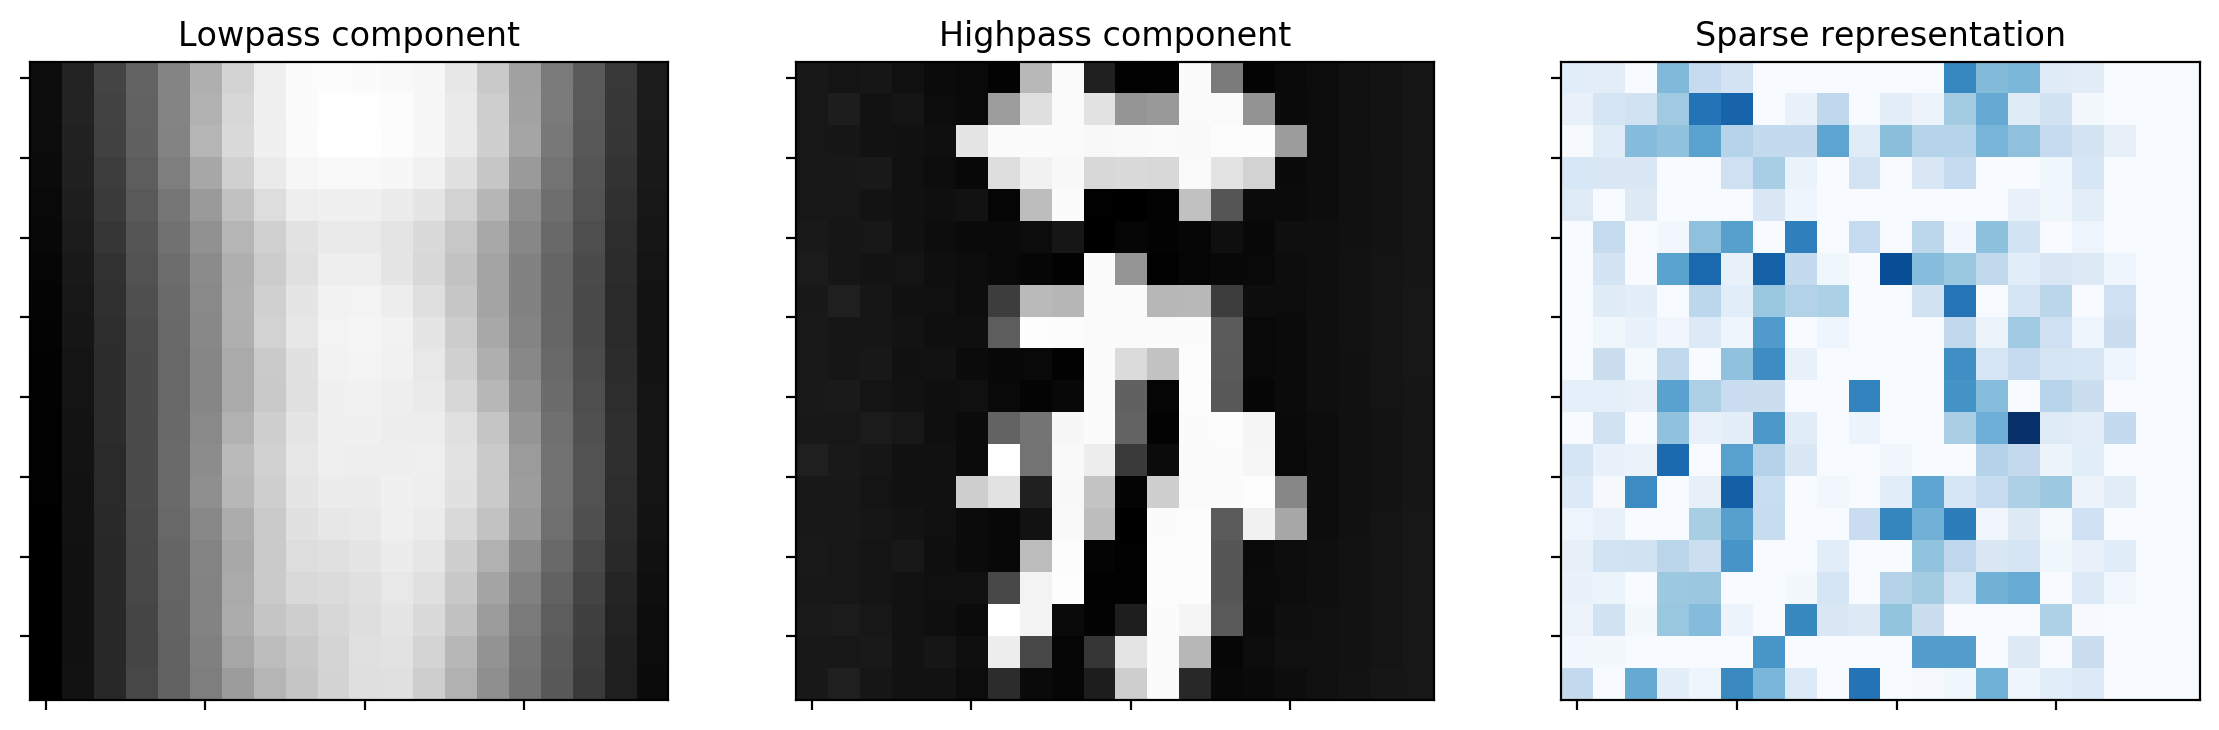
\includegraphics[width=2.5in]{\FIGDIR/CDL_CSC_plot/CCBRPDN_CSC_LHS_comp.png}
\caption{Lowpass, Highpass and Parse representation using single channel CSC with consensus dictionary}
\label{fig_CCBRPDN_CSC_LHS_comp}
\end{figure}

\begin{figure}
\centering
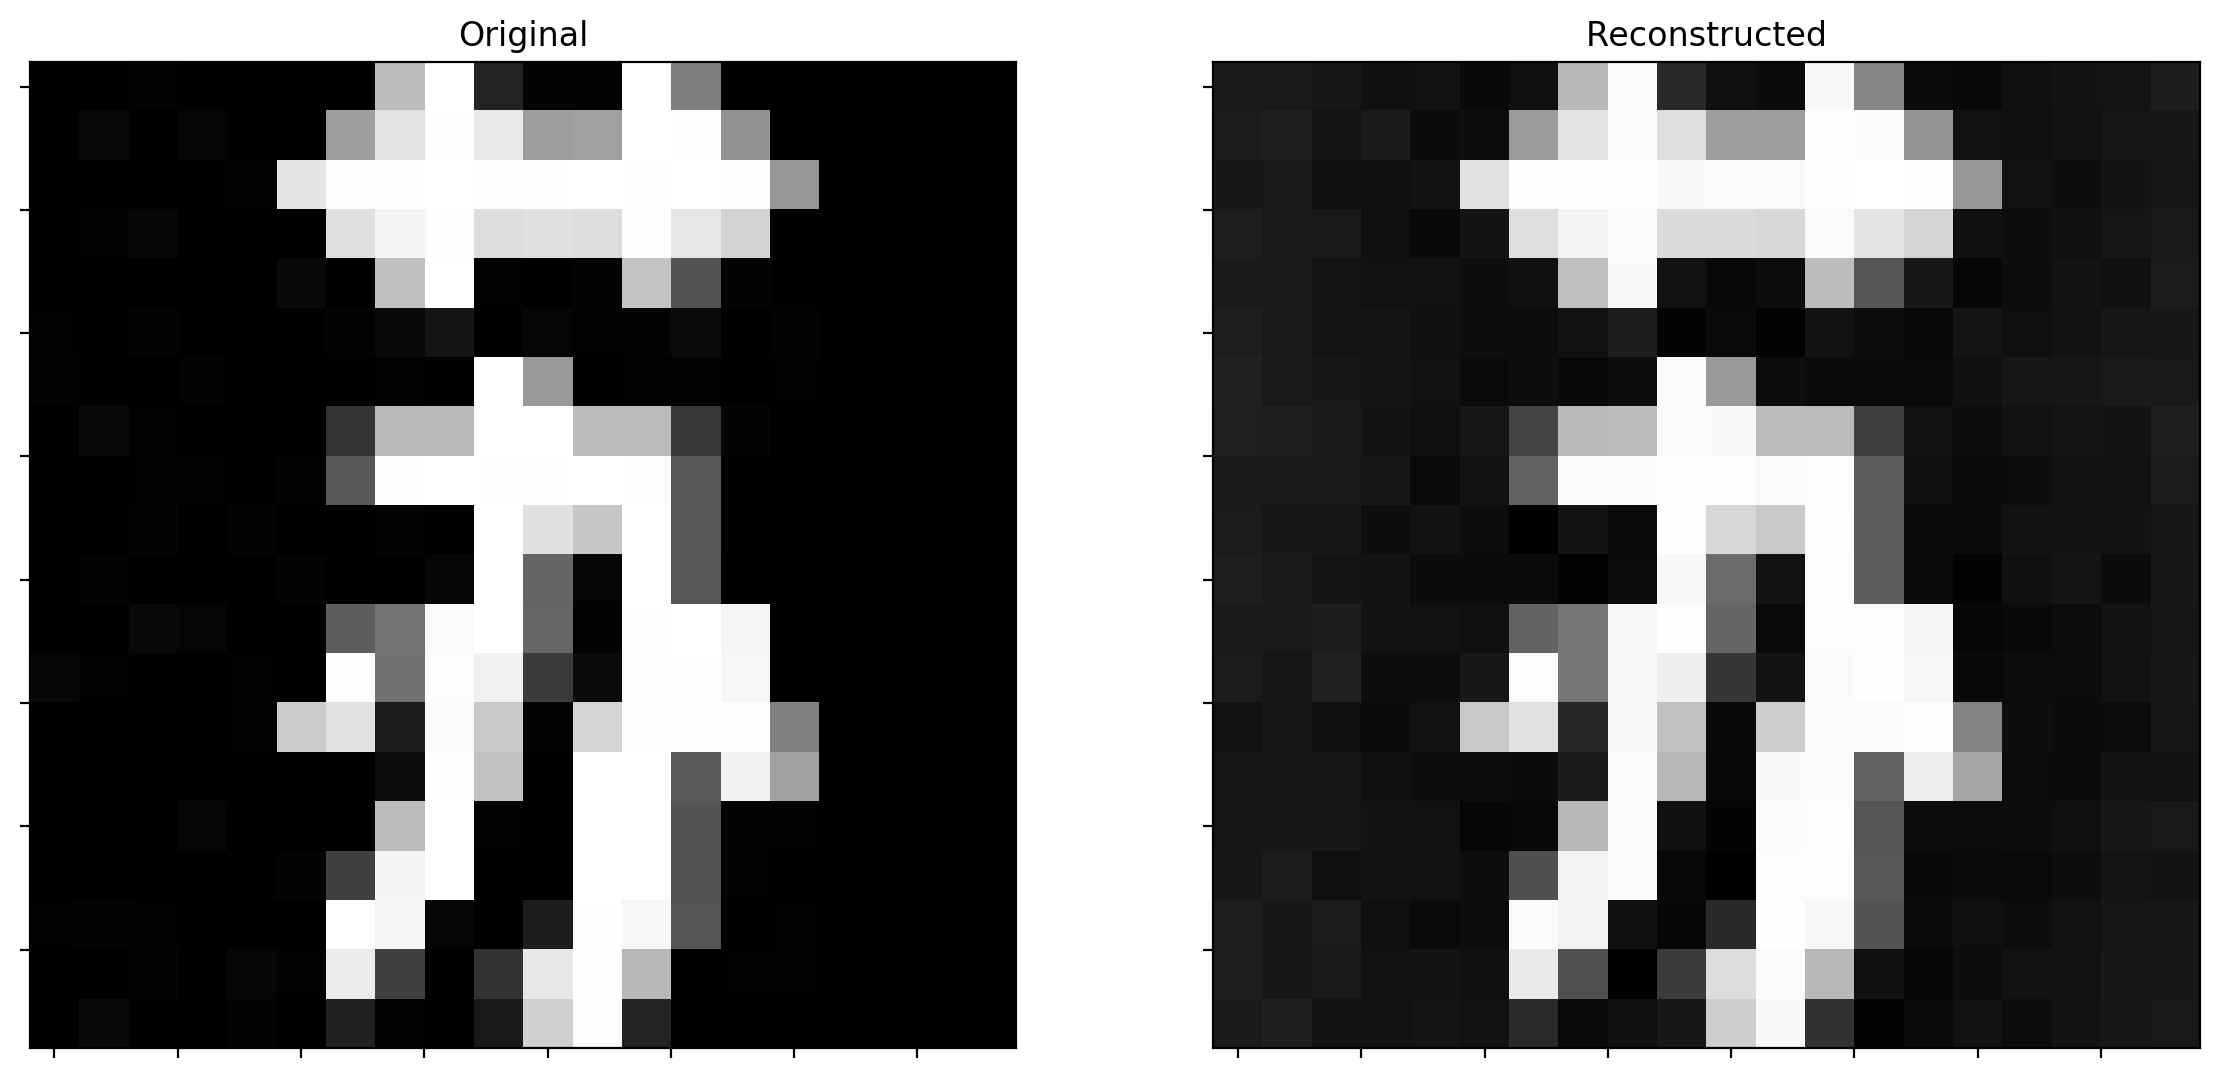
\includegraphics[width=2.5in]{\FIGDIR/CDL_CSC_plot/CCBRPDN_CSC_recon.png}
\caption{Image Reconstruction using single channel CSC with consensus dictionary}
\label{fig_CCBRPDN_CSC_recon}
\end{figure}

\begin{figure}
\centering
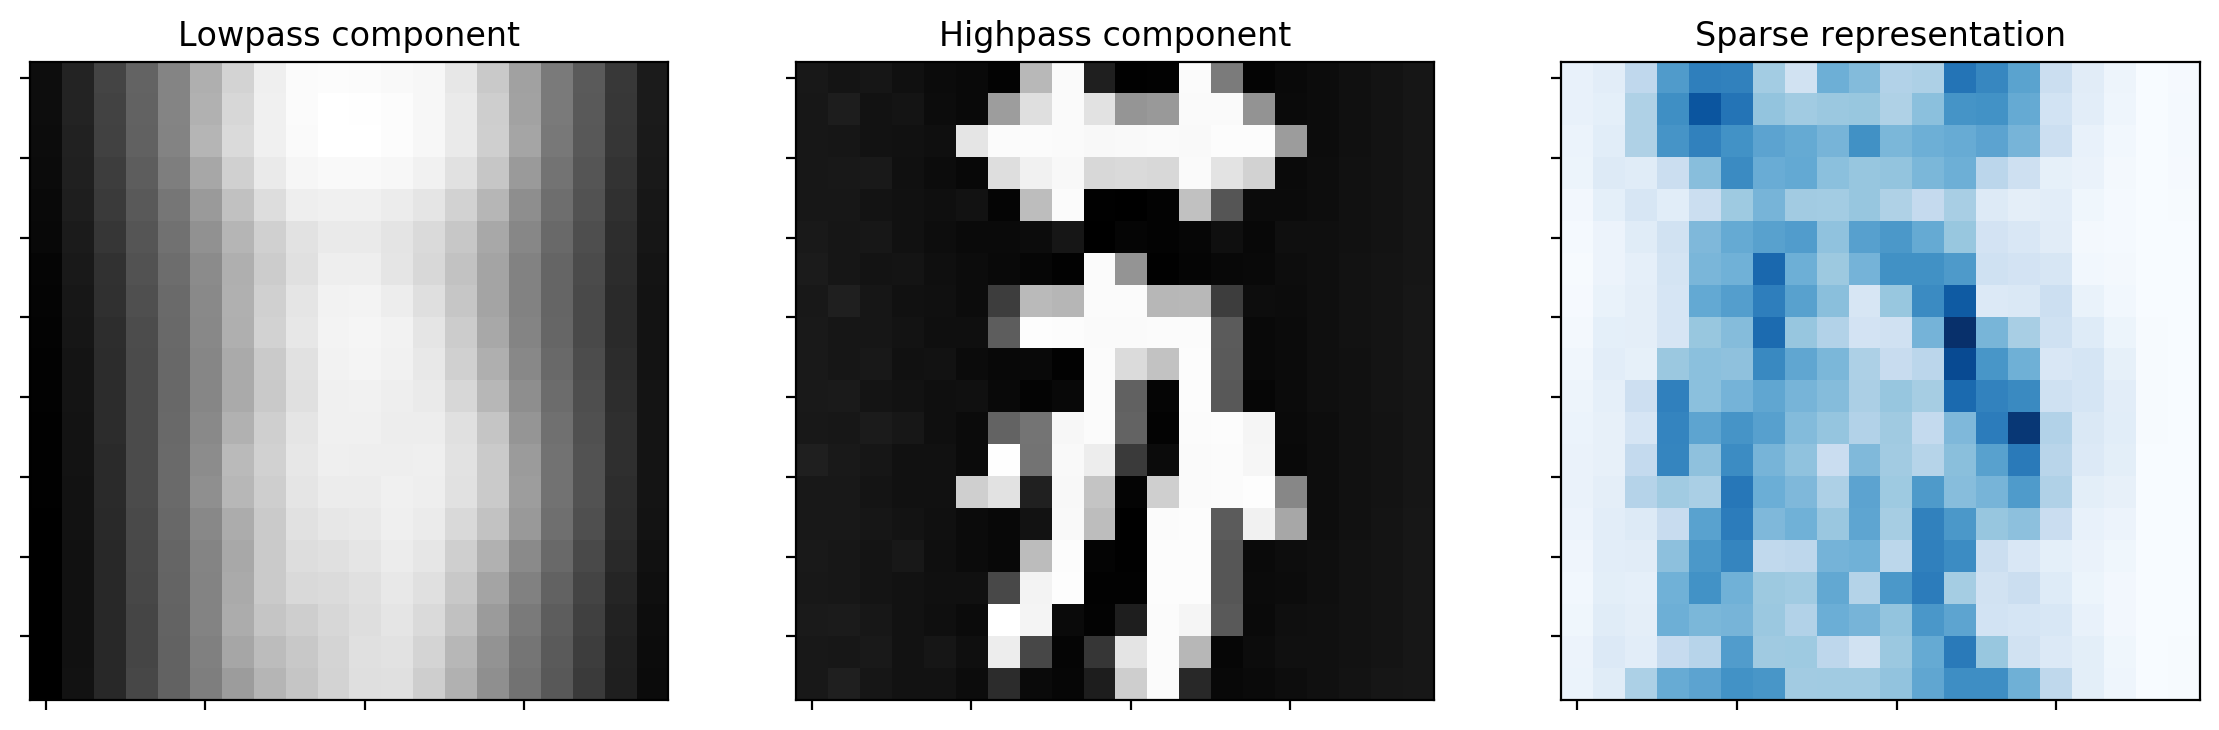
\includegraphics[width=2.5in]{\FIGDIR/CDL_CSC_plot/CCBRPDN_FISTA_LHS_comp.png}
\caption{Lowpass, Highpass and Parse representation using FISTA CSC with consensus dictionary}
\label{fig_CCBRPDN_FISTA_LHS_comp}
\end{figure}

\begin{figure}
\centering
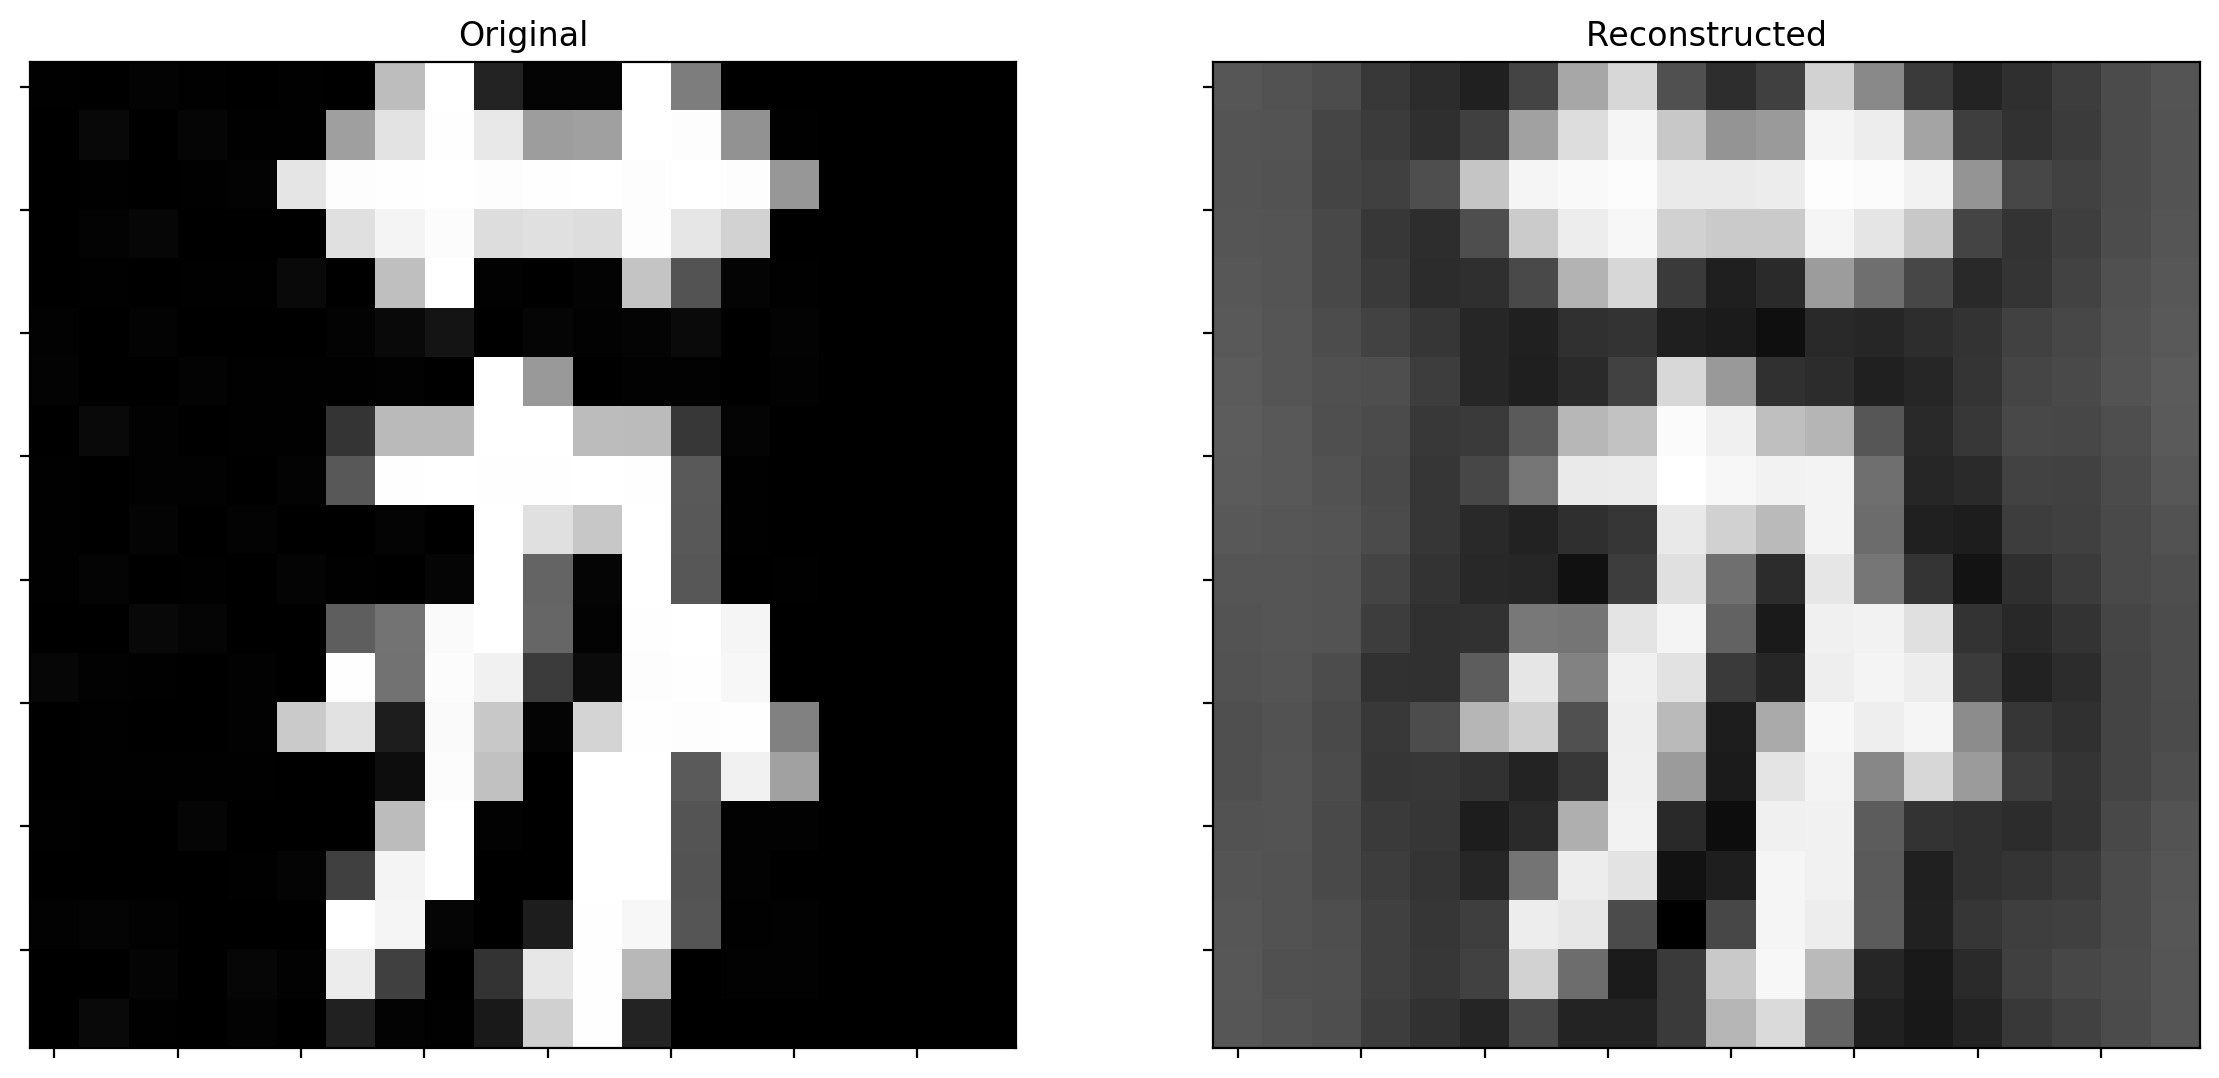
\includegraphics[width=2.5in]{\FIGDIR/CDL_CSC_plot/CCBRPDN_FISTA_recon.png}
\caption{Image Reconstruction using FISTA CSC with consensus dictionary}
\label{fig_CCBRPDN_FISTA_recon}
\end{figure}

\subsection{Decision made after CDL and CSC experiments}
Since there is no significant difference in the CDL algorithms in terms of 
quality of the dictionary. We generate to final dictionaries for each of the
3 classes using the CDL with consensus update since we are dealing with 
over 20000 images and the time saving from allow the consensus is significant.

However, the single channel CSC produce a more ideal sparse representation
and less noisy reconstruction of the images with runtime cost penalty. Since 
it cost less than a second for each image, it is more reasonable to use single
channel CSC to generate the sparse representation for each image instead of the 
FISTA method.

\subsection{CNN Based Training}
After obtaining the sparse representing data as mentioned before, 
we use various ways to classify them. For CNN method, we use both original data 
and sparse representation data to compare their performance in terms of accuracy where
the original data are 20*20 binary character images.
For all the data, we choose 80\% of them as training data and the remain as testing data.
Before feeding to the model, we normalize the original images through dividing them by 255.

\subsubsection{Letter}
\paragraph{Original data} 
The data of category letter consists of 24 letters(except O and I) and 10 digits, 
so the architecture is very simple. After trying several times to find the best architecture.
The best architecture we come up with is to use one convolution layer followed by one dense 
layer as the output layer. 
For the convolution layer, it has 16 kernels since the size of images is not big. 
For the output layer, it has 34 neurons which is corresponding 34 classes and uses softmax as its 
activation function. The softmax function allows for a probabilistic output from 0 to 1. 

The figure \ref{letter_architecture} shows its architecture. 
And when we train the model on the Google Colab GPU, 
the running time of each epoch takes around 0.2s and 
the whole training time is about 10s for 50 epochs.

\begin{figure}[ht]
\centering
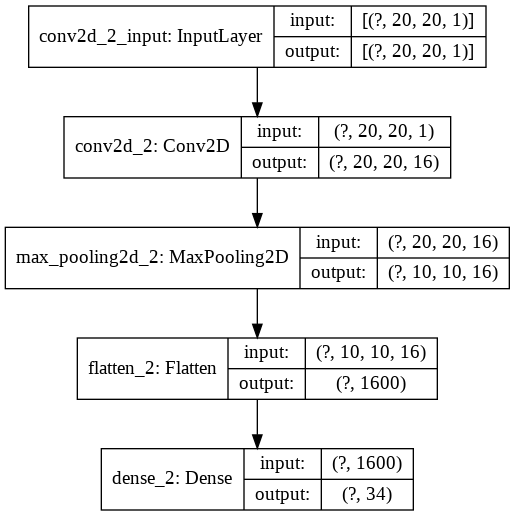
\includegraphics[width=1.5in]{\FIGDIR/04_letter_model.png}
\caption{The architecture of CNN model of letter}
\label{letter_architecture}
\end{figure}

\paragraph{Sparse representing data}
To compare the performance with the original data, we use the same architecture. 
When we use the same device to train the network, the running time of each epoch is around 0.2s 
and the whole training time is about 40s for 200 epochs.

\subsubsection{Area}
\paragraph{Original data} % (fold)
The data of category area consists of 26 letters which is similar to that of letter.
Therefore, we use the same architecture except that for the output layer, 
it only has 26 neurons for its correspond 26 classes. We train the model on the same 
device and each epoch takes around 0.2s and the whole training time is about 10s for 50 epochs.

\paragraph{Sparse representing data}
We use the same model as the original data. The training time for each epoch is the same 
except the total training time is 40s since it has 200 epochs.

\subsubsection{Province}
\paragraph{Original data} % (fold)
The data of category province mainly consist of Chinese character which is not as easy as 
the data of letter to classify them. So after trying different models, we finalize on one 
with a similar architecture is similar to VGG16 \cite{simonyan2014very} which is a famous 
and classic Deep Neural Network architecture and being used in many fields, 
especially in image recognition and classification. We modify the number of kernels since 
the size of our input image is 20*20. We also add some dropout layers to avoid over-fitting. 
Besides that, we also modify the number of neurons of output layers to 31 corresponding to 
31 classes. The figure \ref{original_province_architecture} shows the architecture of the 
network. Each step takes 11ms and 0.15s for each epoch. 
The whole train process takes around 30s for 200 epochs.

\begin{figure}[ht]
\centering
\subfloat{
    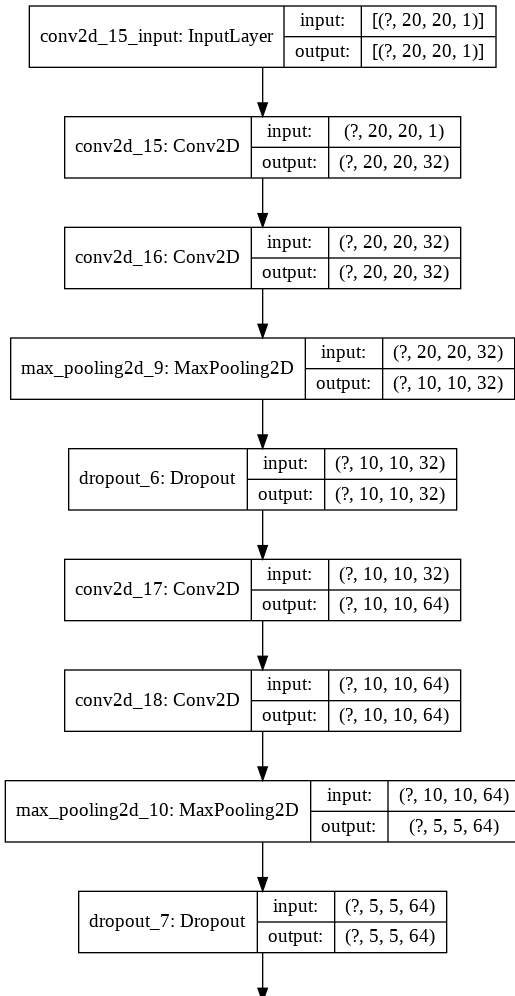
\includegraphics[width=1in]{\FIGDIR/04_province_model.png}
}
\qquad
\subfloat{
    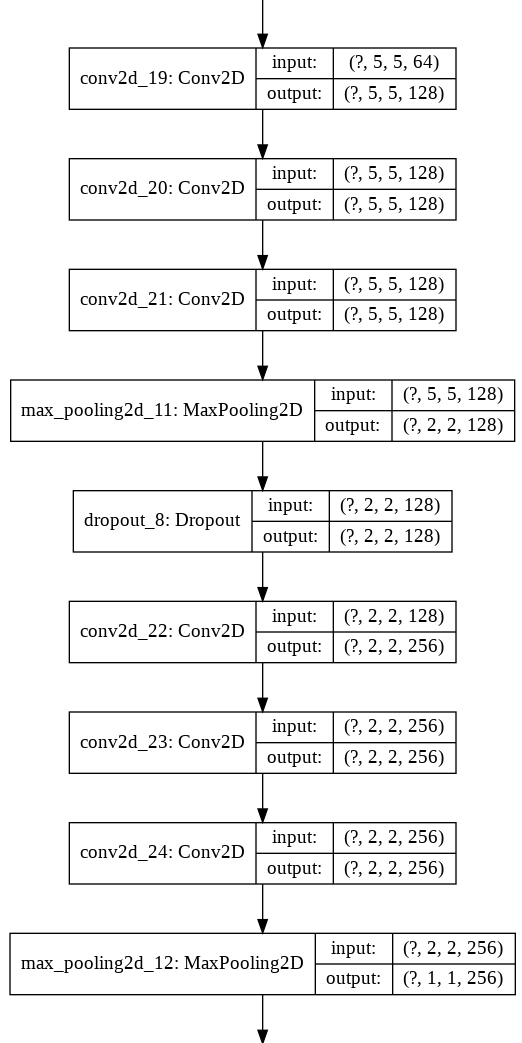
\includegraphics[width=1in]{\FIGDIR/04_province_model2.png}
}
\qquad
\subfloat{
    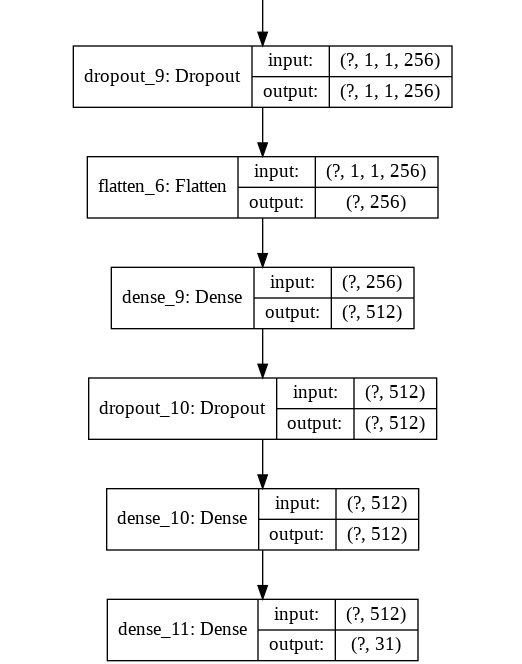
\includegraphics[width=1in]{\FIGDIR/04_province_model3.png}
}
\qquad
\caption{The architecture of original province data}
\label{original_province_architecture}
\end{figure}

\paragraph{Sparse representing data}
The above architecture could not work on these data and the 
result shows if we still use the same architecture, the accuracy will remain 10\%.
The reason may because the the architecture is too deep to the sparse representing data.
After multiple trials, we use two convolution layers which contains 64 kernels and one 
fully-connected layer with 256 neurons. 
The output layer has 31 neurons which is of the same shape.
Figure \ref{ar_pro_sparse} presents the architecture of the model. For the run-time 
performance, each step takes around 6ms and 84ms for each epoch. 
The total training time is 42s for 500 epochs.

\begin{figure}[ht]
\centering
\subfloat{
    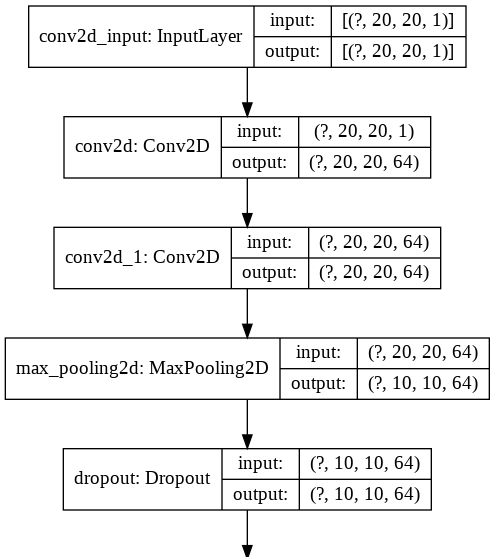
\includegraphics[width=1in]{\FIGDIR/04_province_model_s.png}
}
\qquad
\subfloat{
    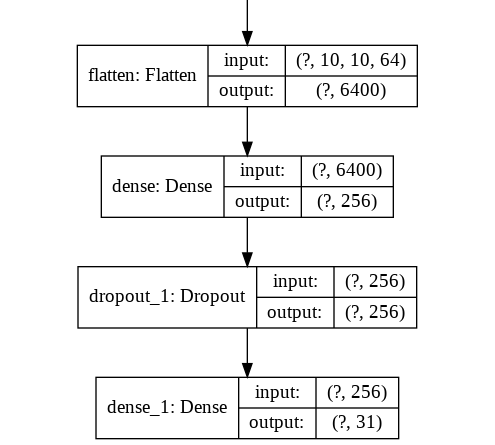
\includegraphics[width=1in]{\FIGDIR/04_province_model_s2.png}
}
\qquad
\caption{The architecture of sparse province data}
\label{ar_pro_sparse}
\end{figure}

\subsection{SVM Based Method}
Besides neuron network, we want to find the performance of using sparse data on some 
classical machine learning methods where SVM appears to be a reasonable option. 
Unlike CNN, SVM doesn't require us to spend time training the model being a classical 
mathematical method, therefore it is more lightweight than neuron networks. 
Before feeding data into the a svm classifier, we have to do PCA on the data because 
the sparse data has a total of 400 features which will take lots of time for SVM to classify them. 
We set the parameter of PCA to 0.9 which means we want to retain 90\% of the variance in the original 
information. For SVM, it has multiple hyper-parameters. 
We have chosen RBF as our kernel function. 
For the parameter C,the regularization parameter, we try multiple C values to find the best one. 
From figure \ref{svm}, we can see the best C values for each category is 3, 2.2 and 2.2 respectively.

\begin{figure}[ht]
\centering
\subfloat[]{
    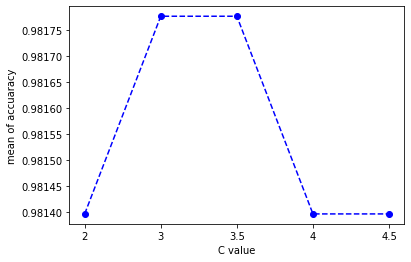
\includegraphics[width=1.2in]{\FIGDIR/04_letter_svm.png}
}
\qquad
\subfloat[]{
    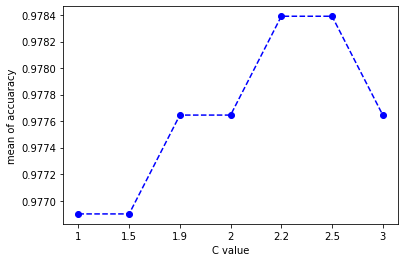
\includegraphics[width=1.2in]{\FIGDIR/04_area_svm.png}
}
\qquad
\subfloat[]{
    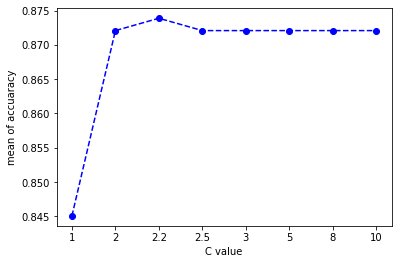
\includegraphics[width=1.2in]{\FIGDIR/04_province_svm.png}
}
\qquad
\caption{(a),(b),(c) respectively shows the mean of accuracy on different C on letter,area and province}
\label{svm}
\end{figure}
